\providecommand{\atd}{..}
\documentclass[../main.tex]{subfiles}

\begin{document}
    \chapter{IFML}\label{ch:ifml}
    \section{Description}\label{sec:description}
    The user will interact with the platform through the interface of a webapp structured in an intuitive way with some explicit references to the functionality of the system. The home page is the starting point of the user interaction flow. It contains the navigation links to the system functionalities and briefly summarizes the system status, i.e. the latest update of the data, the available data sources, the notification of analysis that found a critical issue. All the services available on the platform are authenticated, so the login process must be properly completed before accessing  the application.
    The three main functionalities, accessible from the home, are:
    \begin{itemize}
        \item \textbf{Search}
        \item \textbf{Automated Analysis}
        \item \textbf{Dashboards}
    \end{itemize}
    The search is a feature that allows to extract information and conduct studies by specifying filters like data sources, time range, geographic areas and visualizations. This process can involve several refining operations of the constraints defined in order to obtain a significant result: that is the reason why the page in which the filters are selected and the one where we see the results is exactly the same. Obviously at the beginning all the page is occupied by the filters, and after running the search the majority of the page will be occupied from the results while the filters will be accessible on the side of the screen.
    The analysis section instead contains a collection of the analyzes already created by the users in the system. From that page, it’s possible to reach a more detailed page showing the information of a single analysis, like the latest results, the time taken to run it, who created it and so on. In the context of the application, an analysis is intended as a specific search launched on some data which is saved and is updated in the background periodically. That’s the reason why the creation of an analysis starts from the definition of a search. e.g. of analysis can be a search that runs every weekend right after the football matches, extracts the information about the usage of public transport services and traffic around the stadium, and throws a notification in case a certain threshold is reached.
    The dashboard section allows the creation and visualization of a dashboard. A dashboard is a report composed by panels where each panel shows the result of a search. Perhaps a search can be also saved as a “dashboard panel”. Thus dashboards allow having a global view of some aggregated data by time and issue category, the detail of which can be viewed through a tabular or graphic interface. For example, it’s possible to create a dashboard about big music events, that shows in the panels information about how the people behaved going to the concert and how the people moved after the concert, for example divided per transport categories. The dashboard can be saved and viewed to learn important information when organizing the security of other events.

    \section{IFML Diagram}\label{sec:ifml-diagram}
    Due to the space limitation of the pdf, in order to correctly view the entire IFML diagram please refer to the \href{https://miro.com/app/board/o9J_kuKN_dk=/}{\textit{Miro Link}}.
    \\
    \\
    \begin{figure}[H]
        \centering
        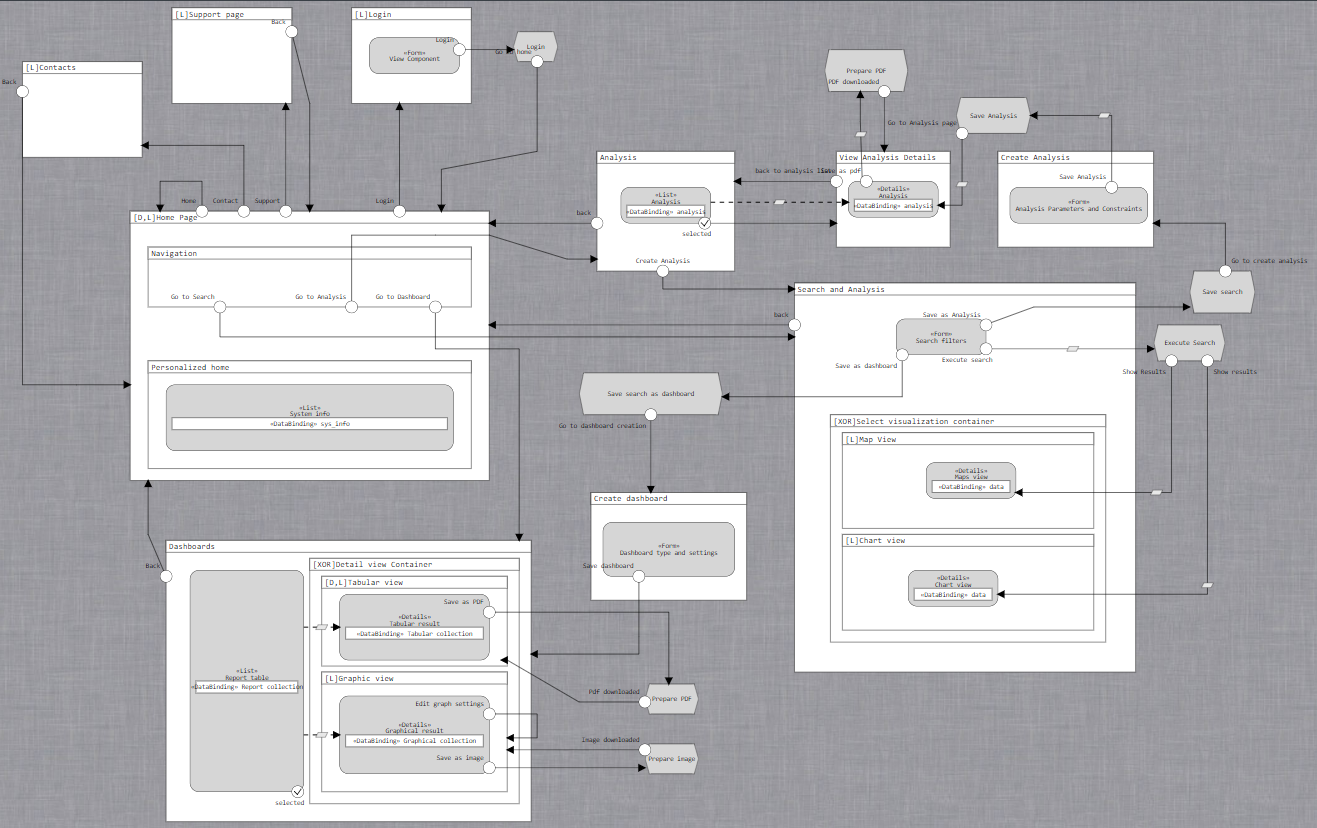
\includegraphics[scale = 1.5]{assets/ifml/ifml_sum.png} \\
        \caption[]{Overview of the IFML}\label{fig:figure4}
    \end{figure}
    \chapter{Wireframes}\label{ch:wireframes}
    \section{Description}\label{sec:description2}
    With the wireframes we wanted to show the navigation flow, how the system behave while performing searches and the connection that there is between the search and the dashboards. In the home we can see the navigation menu and a section that is customizable, showing system information or a pre-selected dashboard. Starting from the navigation menu we can go to the search page, where we can insert the filters. Once we are done, we can run the search: what happens is that the page remains the same, but the content changes. In fact the filters will be still accessible on the right side of the page in order to refine the search, but the main object of the page are now the results. Speaking about visualizations, is possible to change the way results are displayed, using for example maps or charts, but even if the content changes, the page will always remain the same. Then, starting from the generated search results is possible to set up an analysis or create a dashboard panel, and thus being redirected to the dashboard section.
    \section{Wireframes}\label{sec:wireframes-screen}
    \begin{figure}[H]
        \centering
        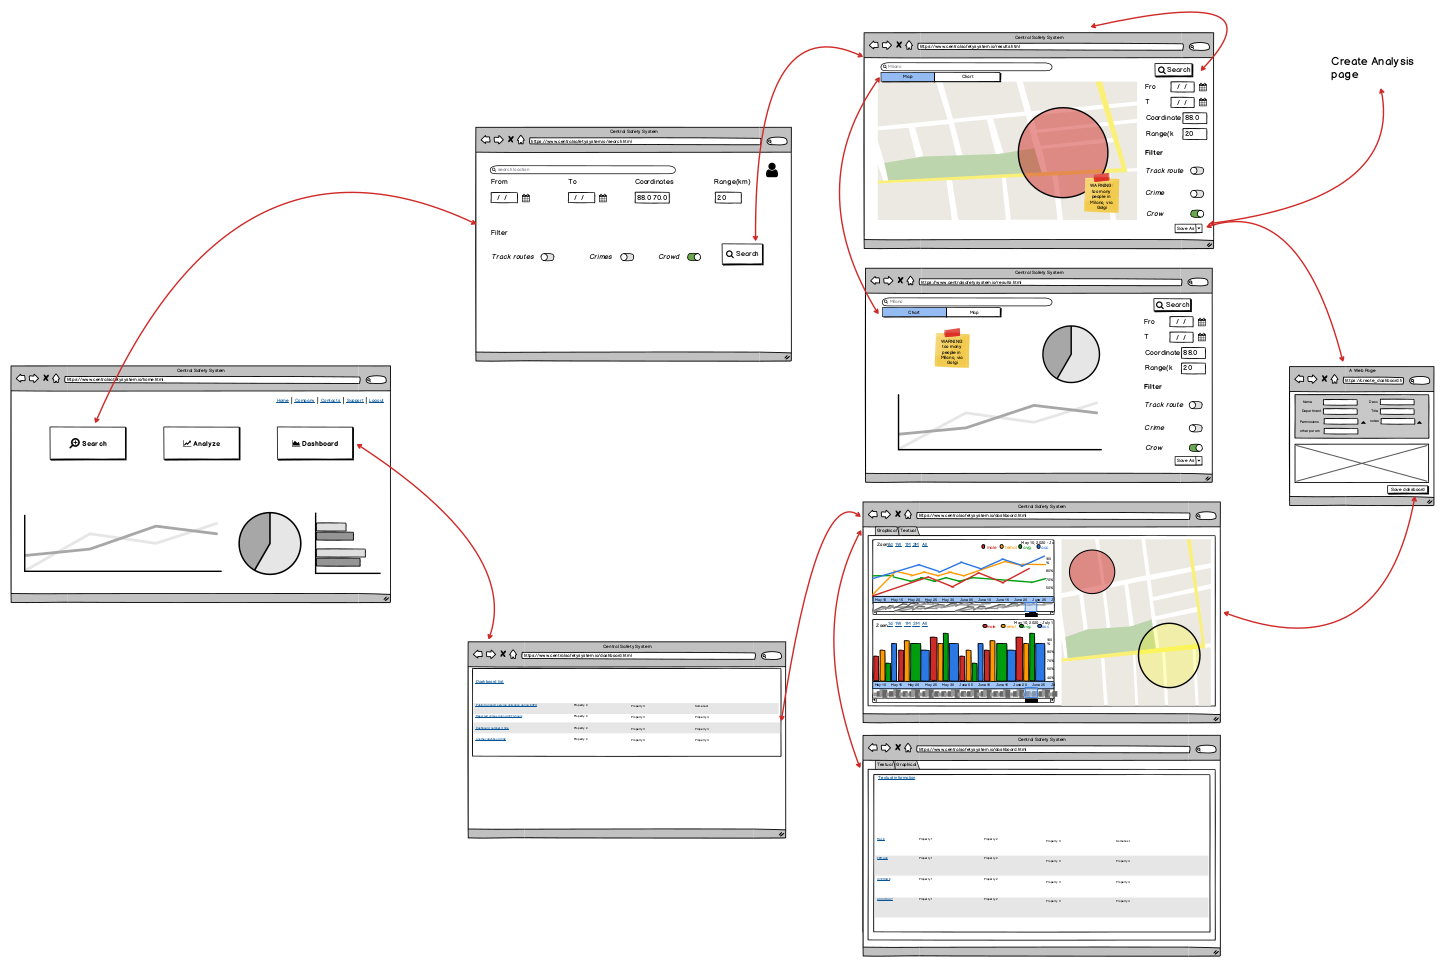
\includegraphics[scale = 0.35]{assets/wireframes/wire_sum.png} \\
        \caption[]{Overview of the wireframes}\label{fig:figure5}
    \end{figure}
    \begin{figure}[H]
        \centering
        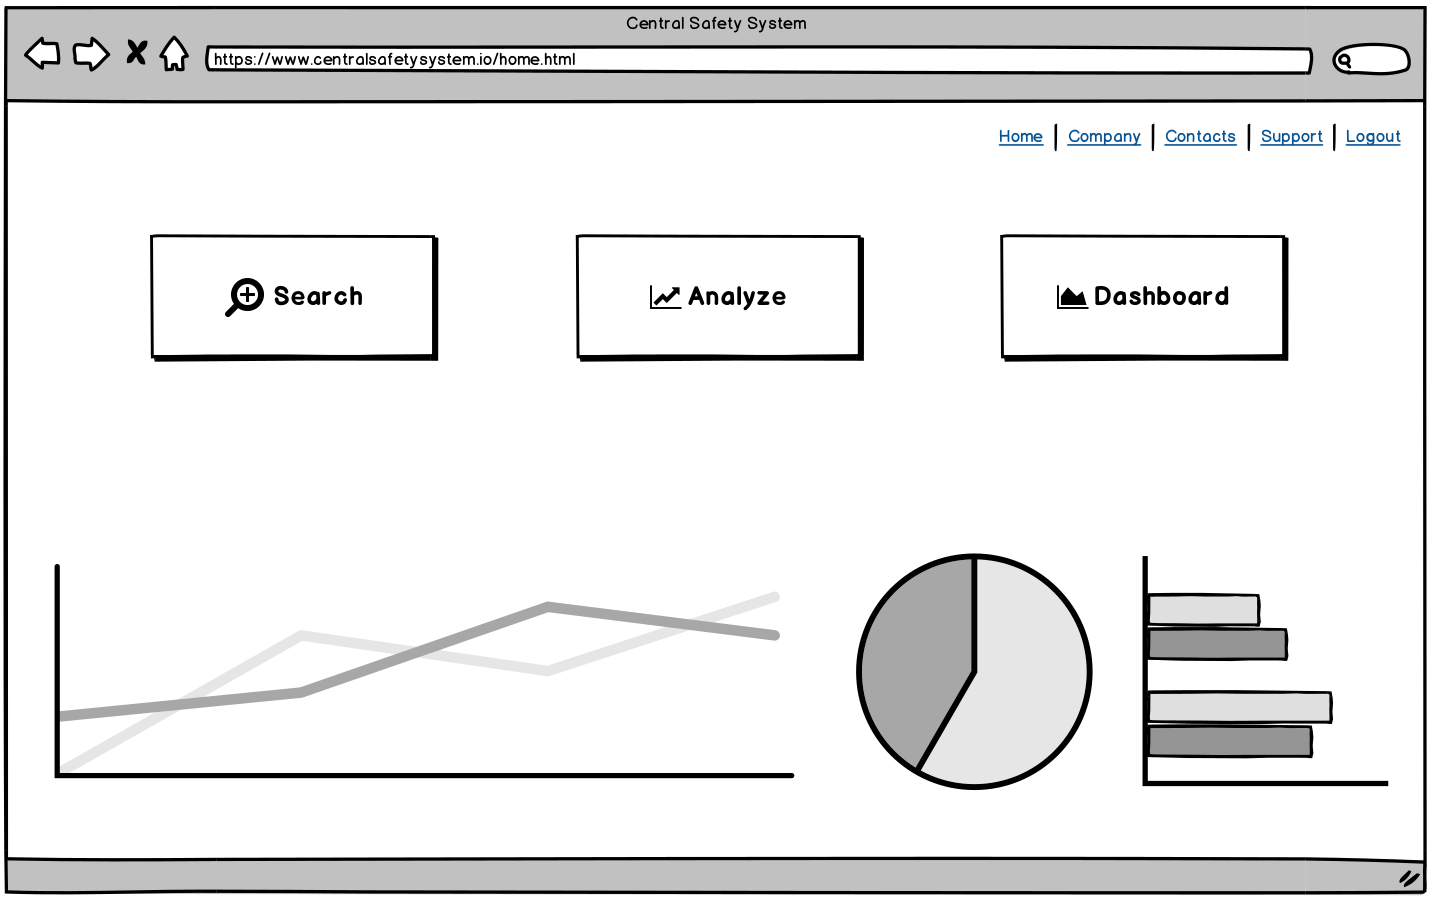
\includegraphics[scale = 0.32]{assets/wireframes/wire1.png} \\
        \caption[]{Home Page}\label{fig:figure6}
    \end{figure}
    \begin{figure}[H]
        \centering
        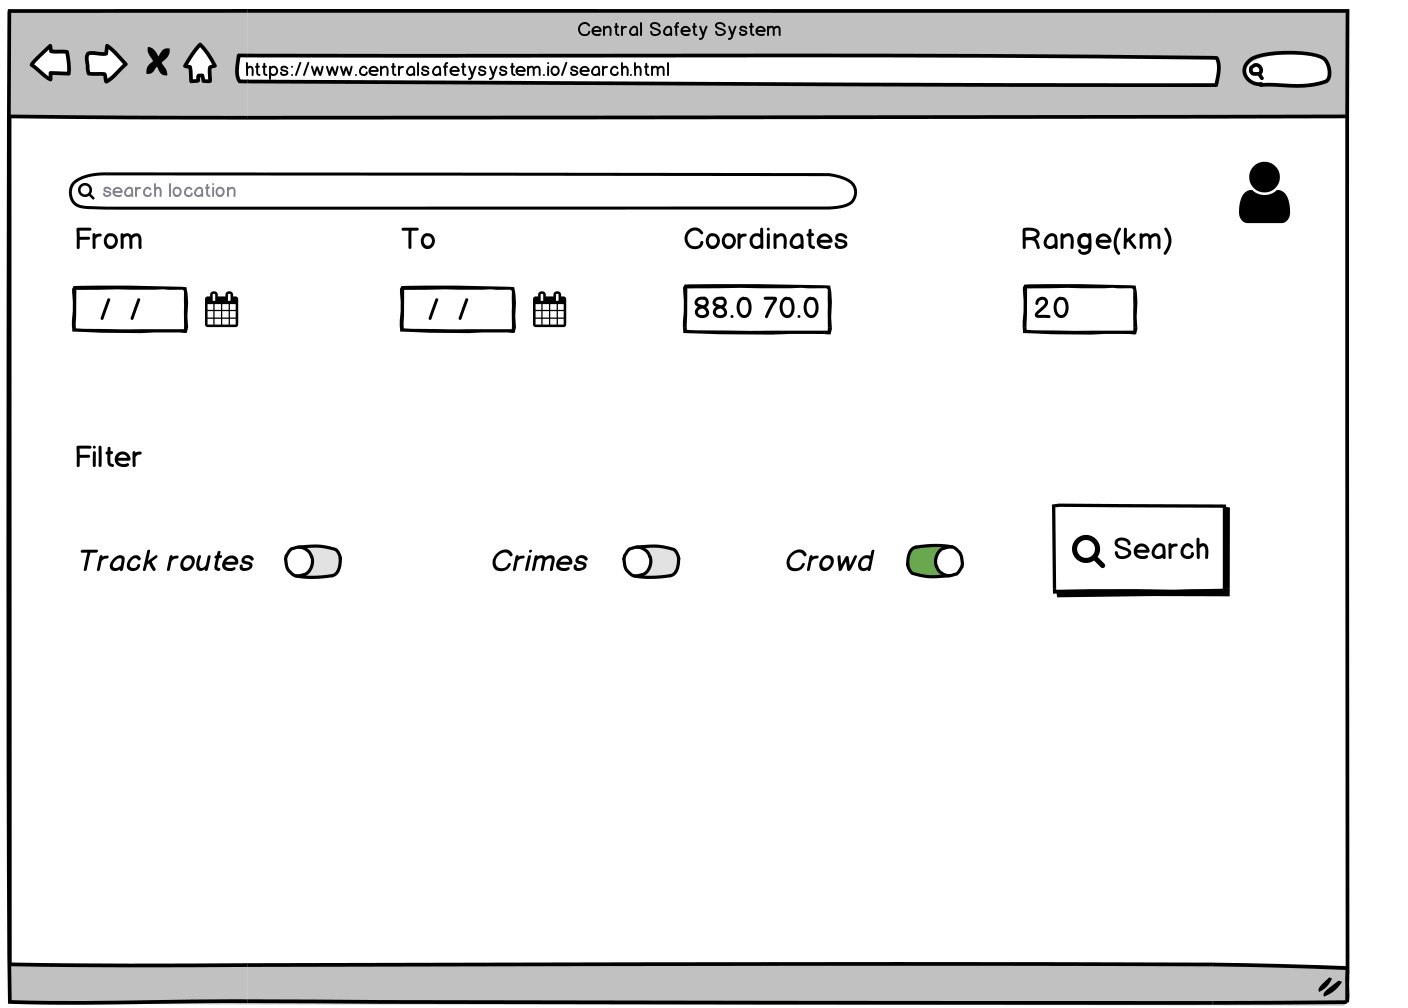
\includegraphics[scale = 0.33]{assets/wireframes/wire2.png} \\
        \caption[]{Search Page}\label{fig:figure7}
    \end{figure}
    \begin{figure}[H]
        \centering
        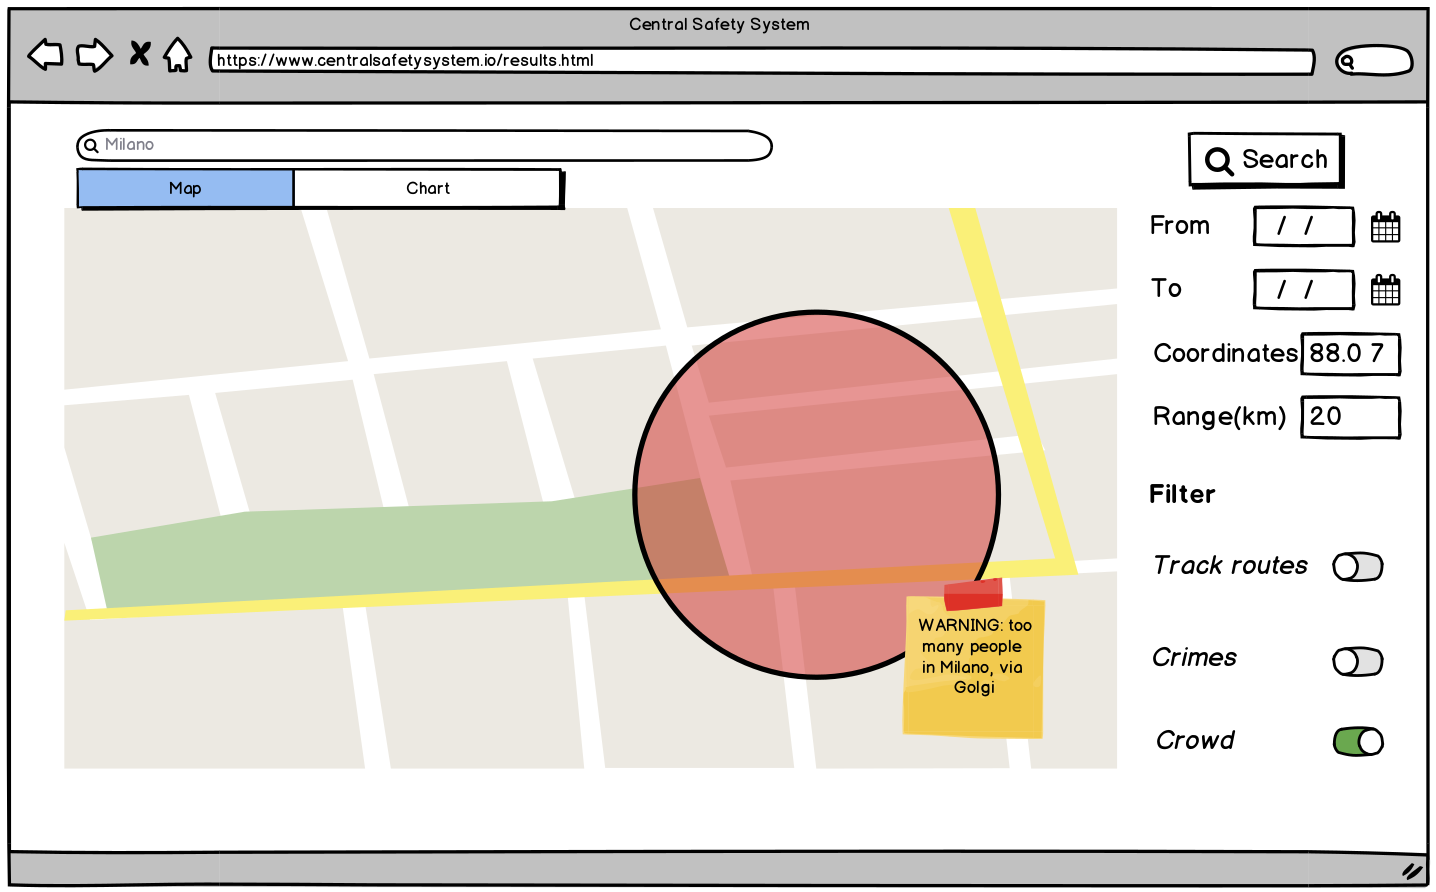
\includegraphics[scale = 0.33]{assets/wireframes/wire3.png} \\
        \caption[]{After Search Page, Map view}\label{fig:figure8}
    \end{figure}
    \begin{figure}[H]
        \centering
        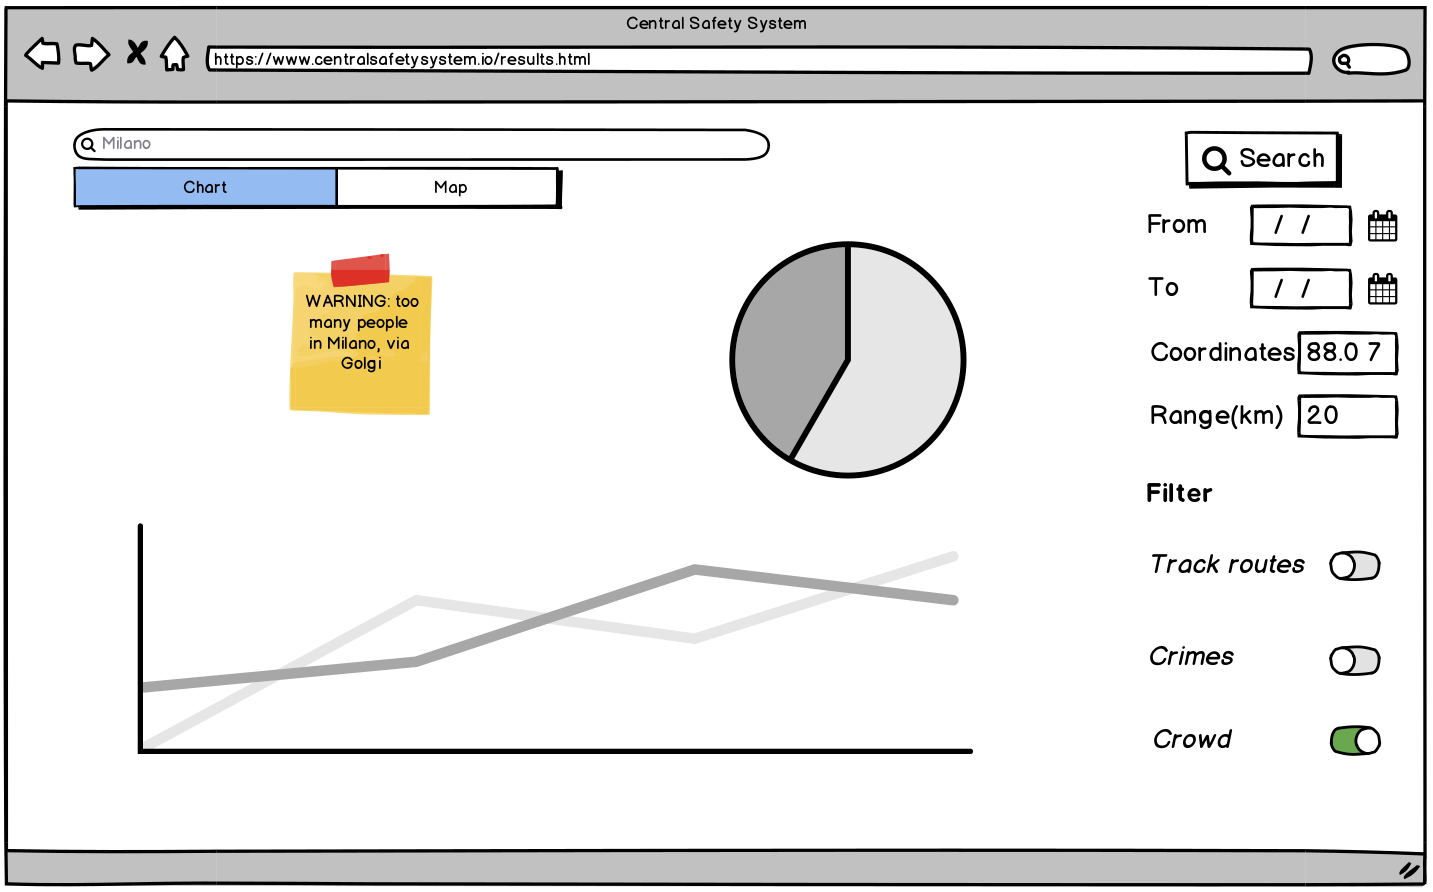
\includegraphics[scale = 0.33]{assets/wireframes/wire4.png} \\
        \caption[]{After Search Page, Charts view}\label{fig:figure9}
    \end{figure}
    \begin{figure}[H]
        \centering
        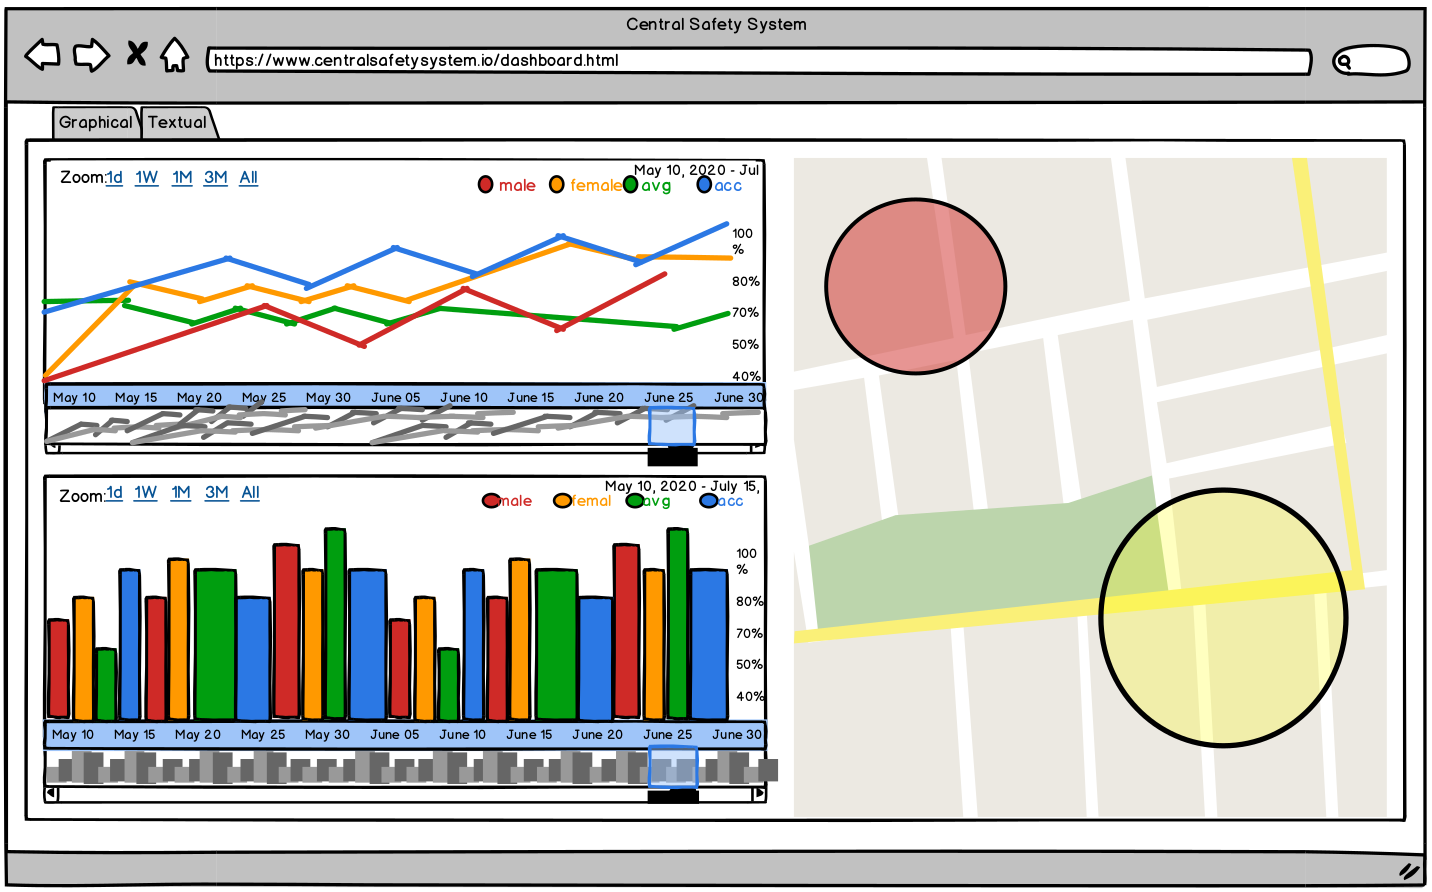
\includegraphics[scale = 0.33]{assets/wireframes/wire5.png} \\
        \caption[]{Graphical Dashboard}\label{fig:figure10}
    \end{figure}
    \begin{figure}[H]
        \centering
        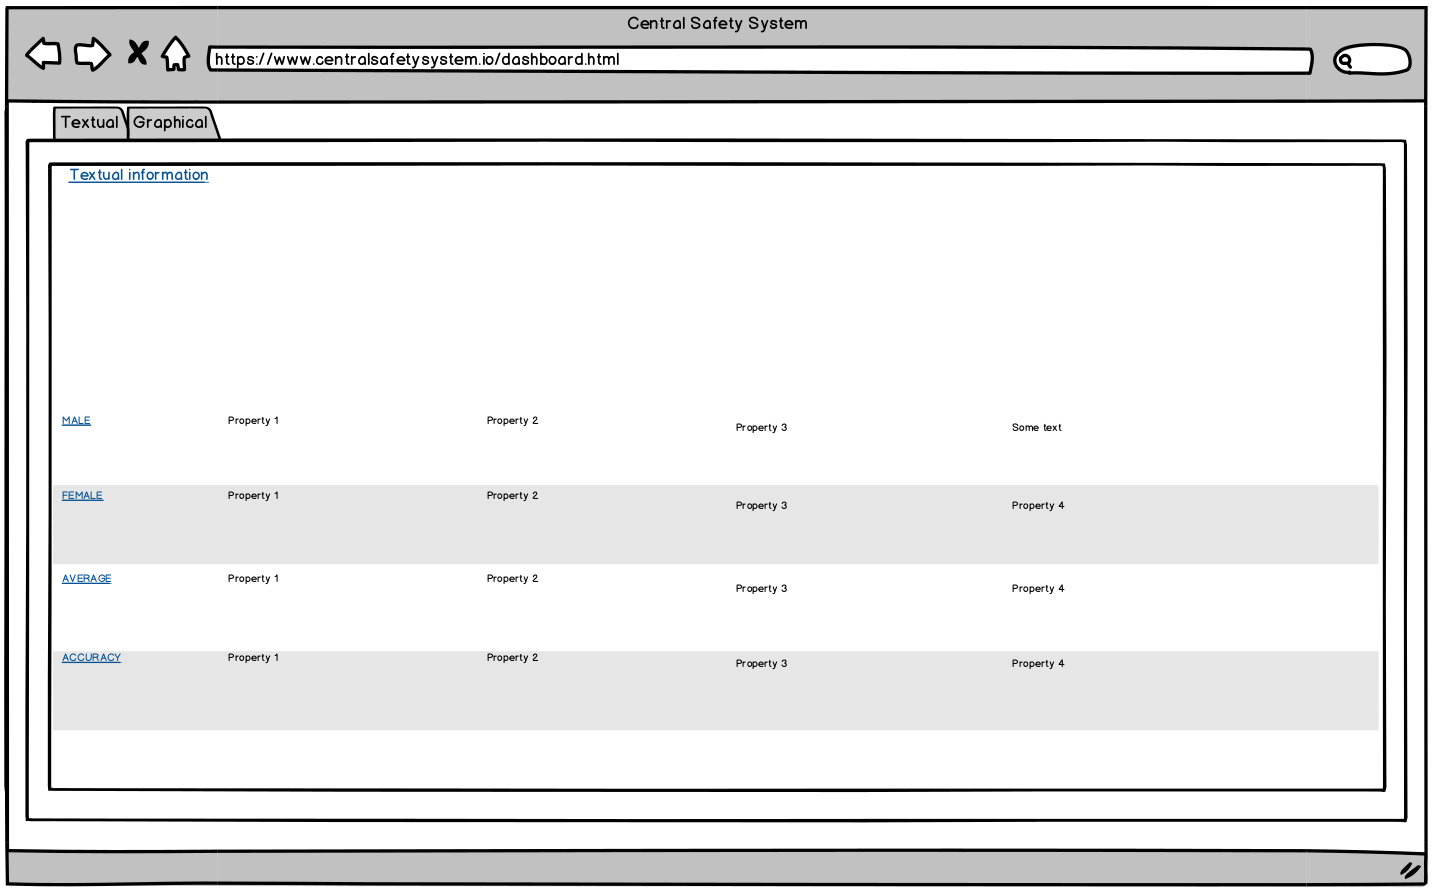
\includegraphics[scale = 0.33]{assets/wireframes/wire6.png} \\
        \caption[]{Textual Dashboard}\label{fig:figure11}
    \end{figure}
    \begin{figure}[H]
        \centering
        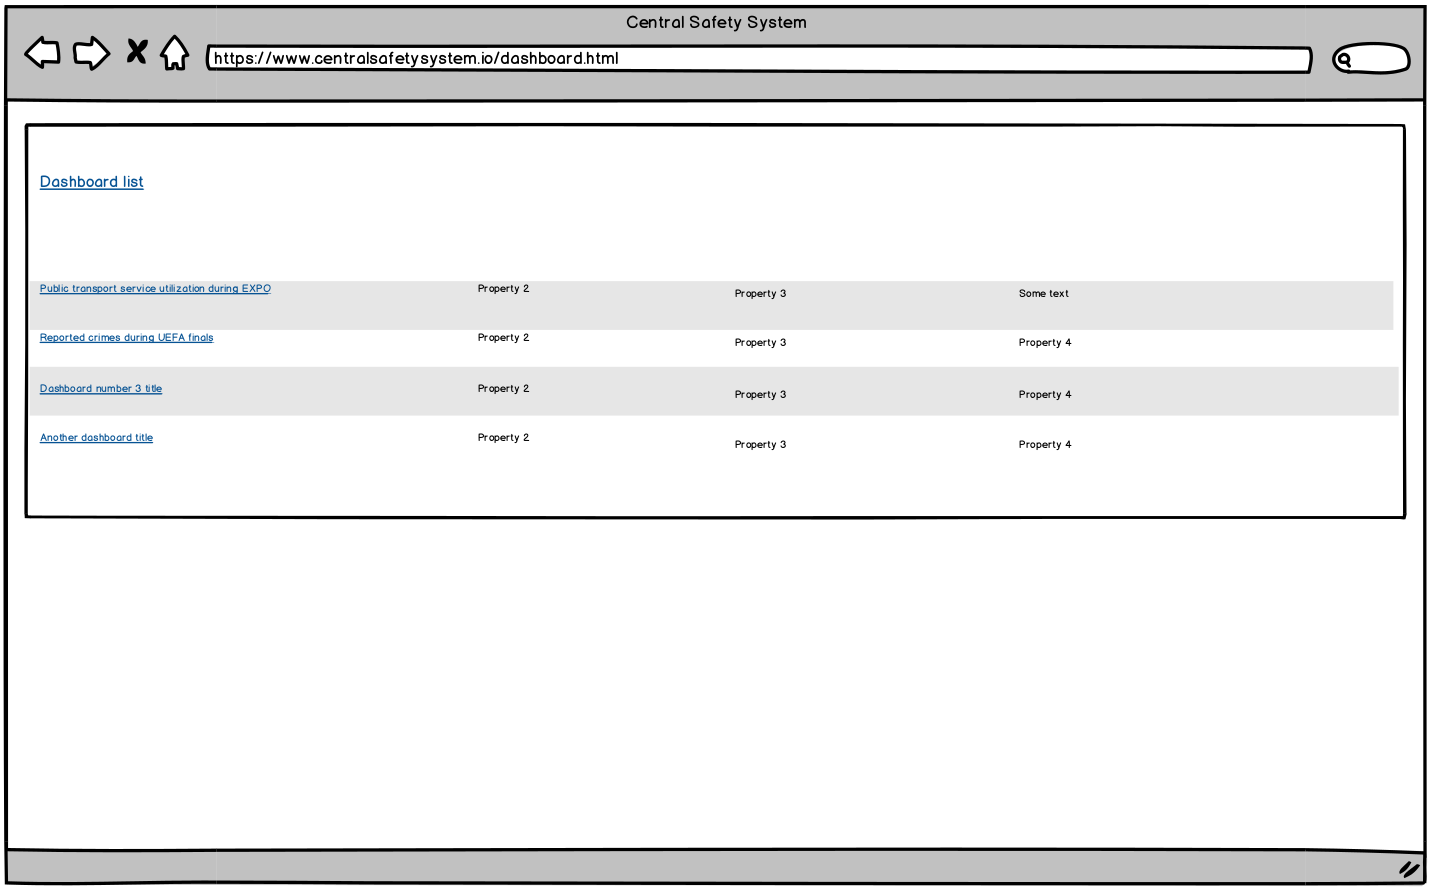
\includegraphics[scale = 0.33]{assets/wireframes/wire7.png} \\
        \caption[]{Dashboards List}\label{fig:figure12}
    \end{figure}

    \chapter{Mockups}\label{ch:mockups}
    \section{Description}\label{sec:description3}
    Finally, with the mockups we wanted to show a possible interface used in the search pages. We have chosen to maintain a clean and modern UI, in order to make the user comfortable while using the system. The form that allows to interact with the filters must be intuitive enough to allow the user to perform searches without having to use a query language.
    Once the search is launched, the results appear and the filters move on the right. In this mockup we are showing a possible visualization through a map, with the system highlighting the results using graphical objects and text messages.
    Using a menu, it is possible to choose among different visualizations. Here we have proposed for example a chart that highlights how the crowd has changed over time and the peak value registered.
    \section{Mockups}
    The full Mockups of submission 07 are available \href{https://invis.io/P3X4WSWR7JS#/417983015_Homepage}{\textit{HERE}}
    \begin{figure}[H]
        \centering
        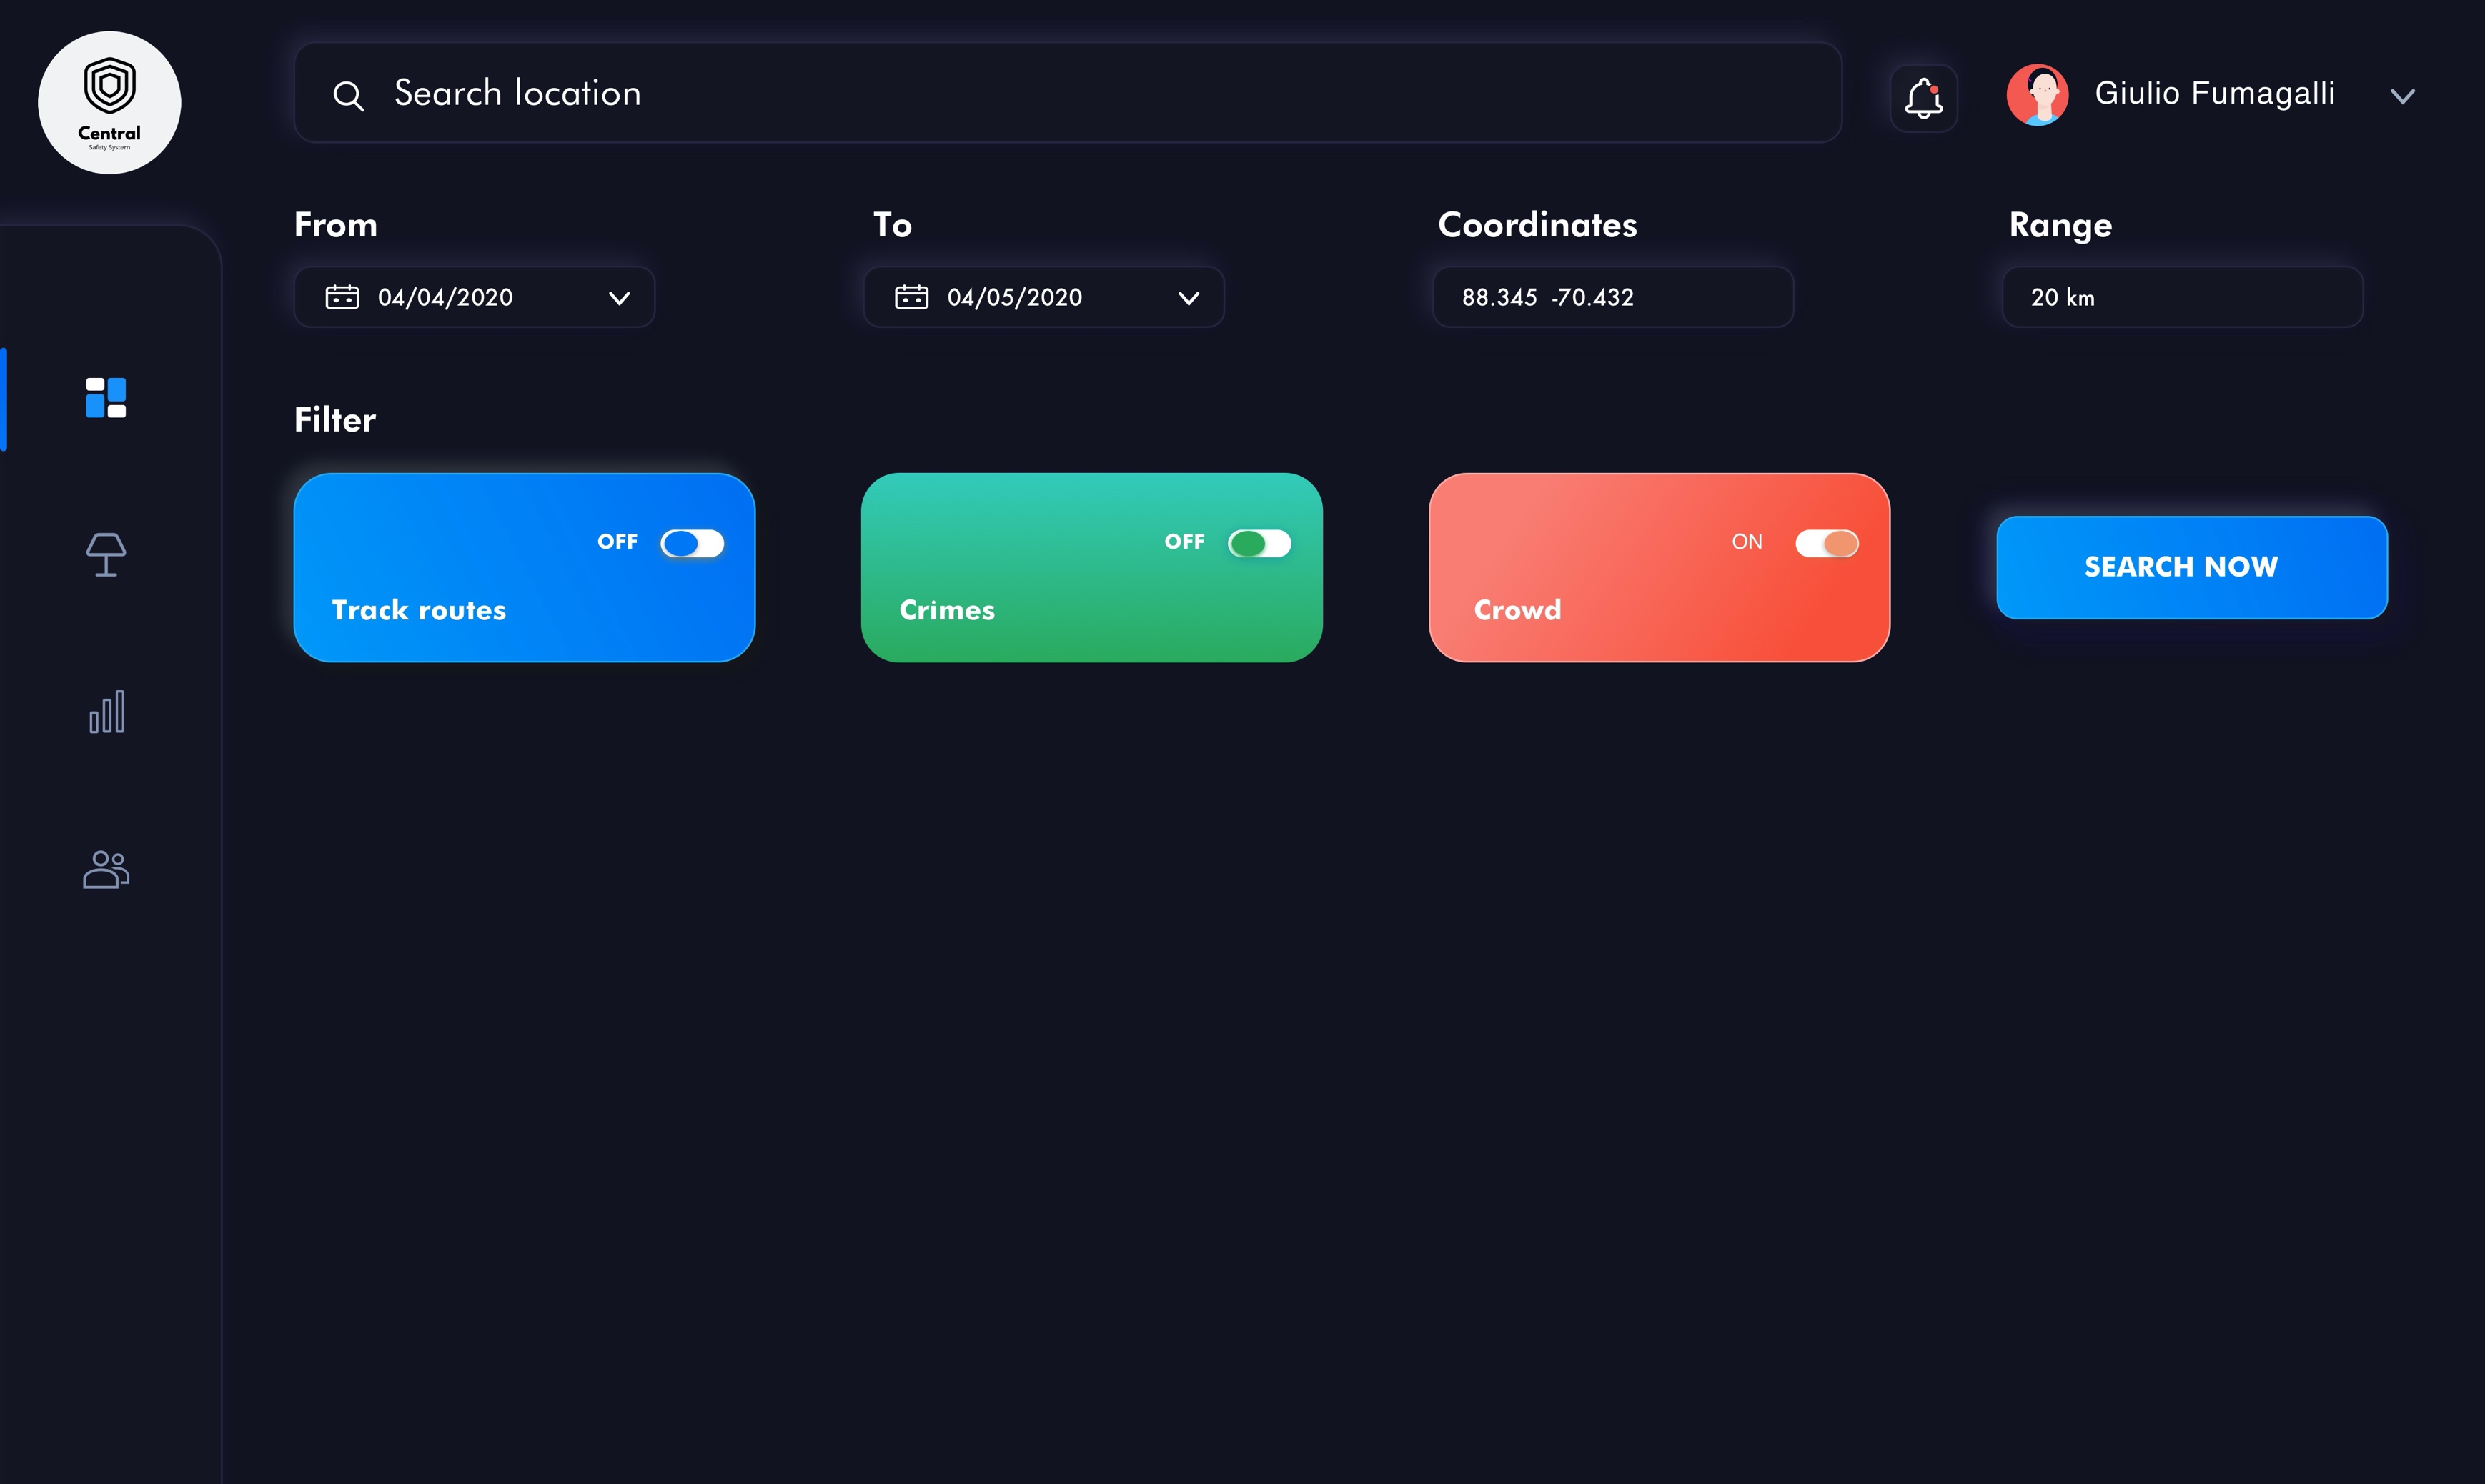
\includegraphics[scale = 0.6]{assets/mockups/mock_search.png}\\
        \caption[]{Search Page}\label{fig:figure}
    \end{figure}
    \begin{figure}[H]
        \centering
        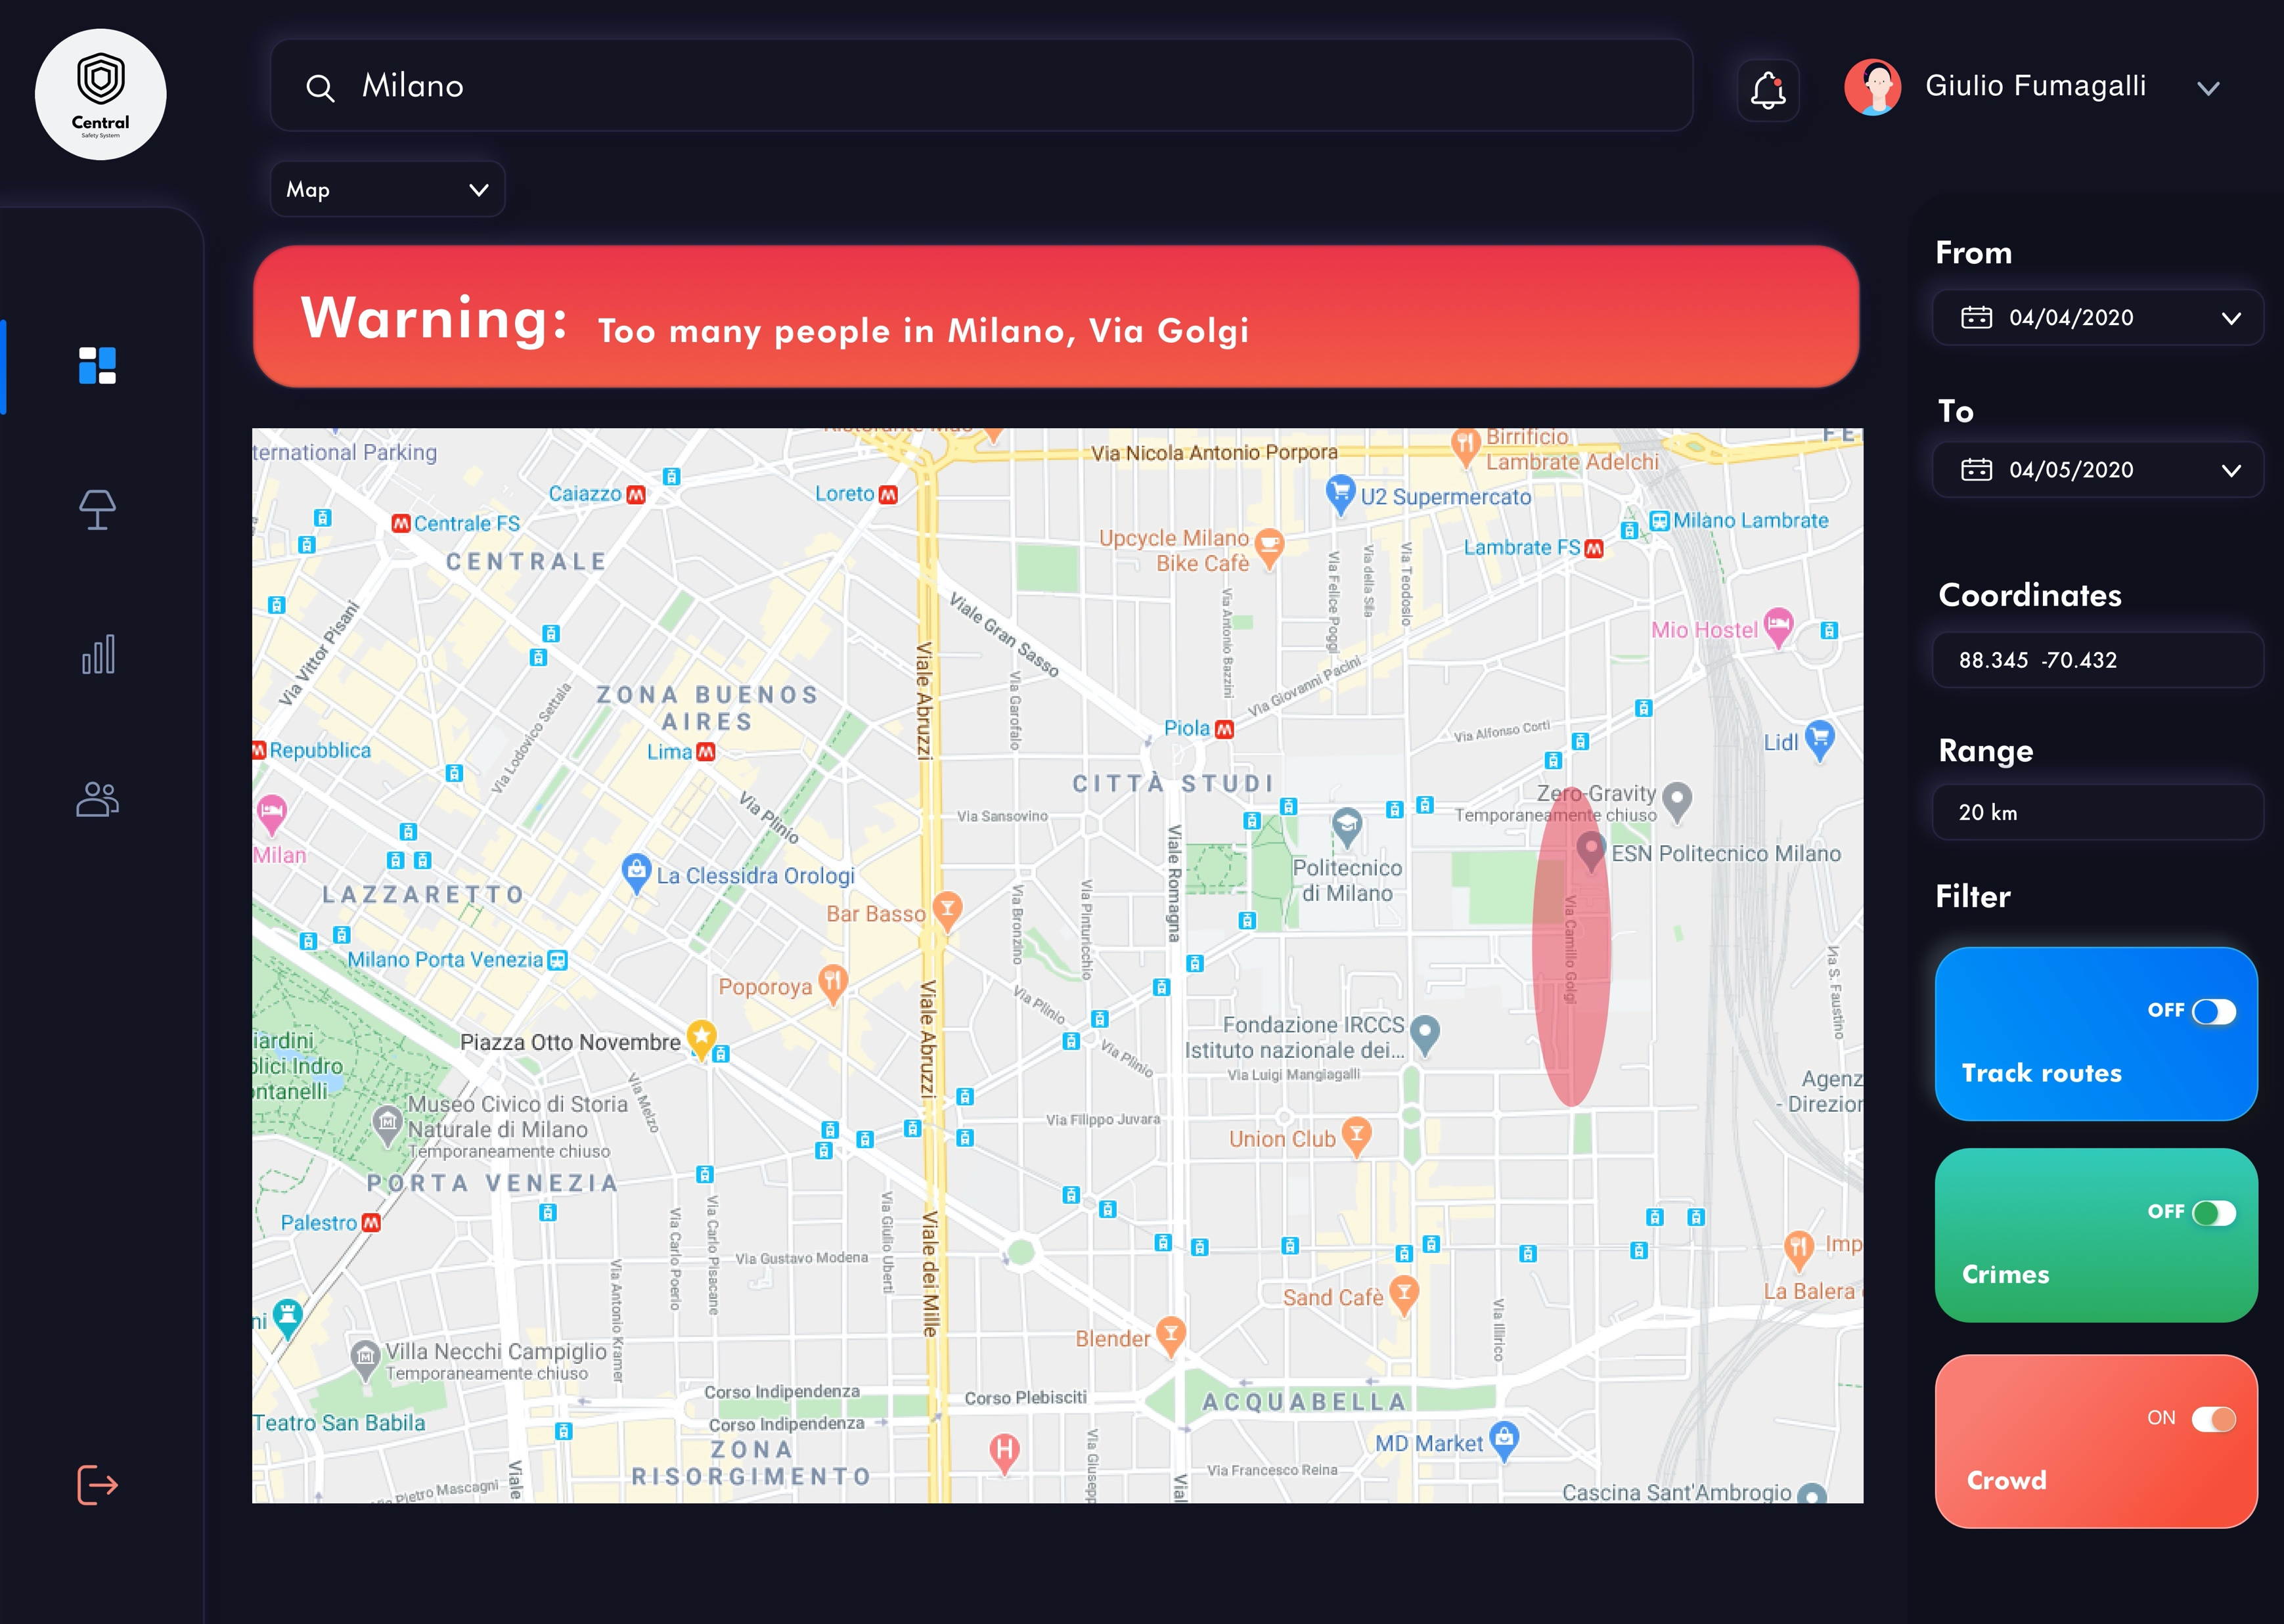
\includegraphics[scale = 0.6]{assets/mockups/mock_aftersearch.png}\\
        \caption[]{After Search Page}\label{fig:figure2}
    \end{figure}
    \newpage
    \begin{figure}[H]
        \centering
        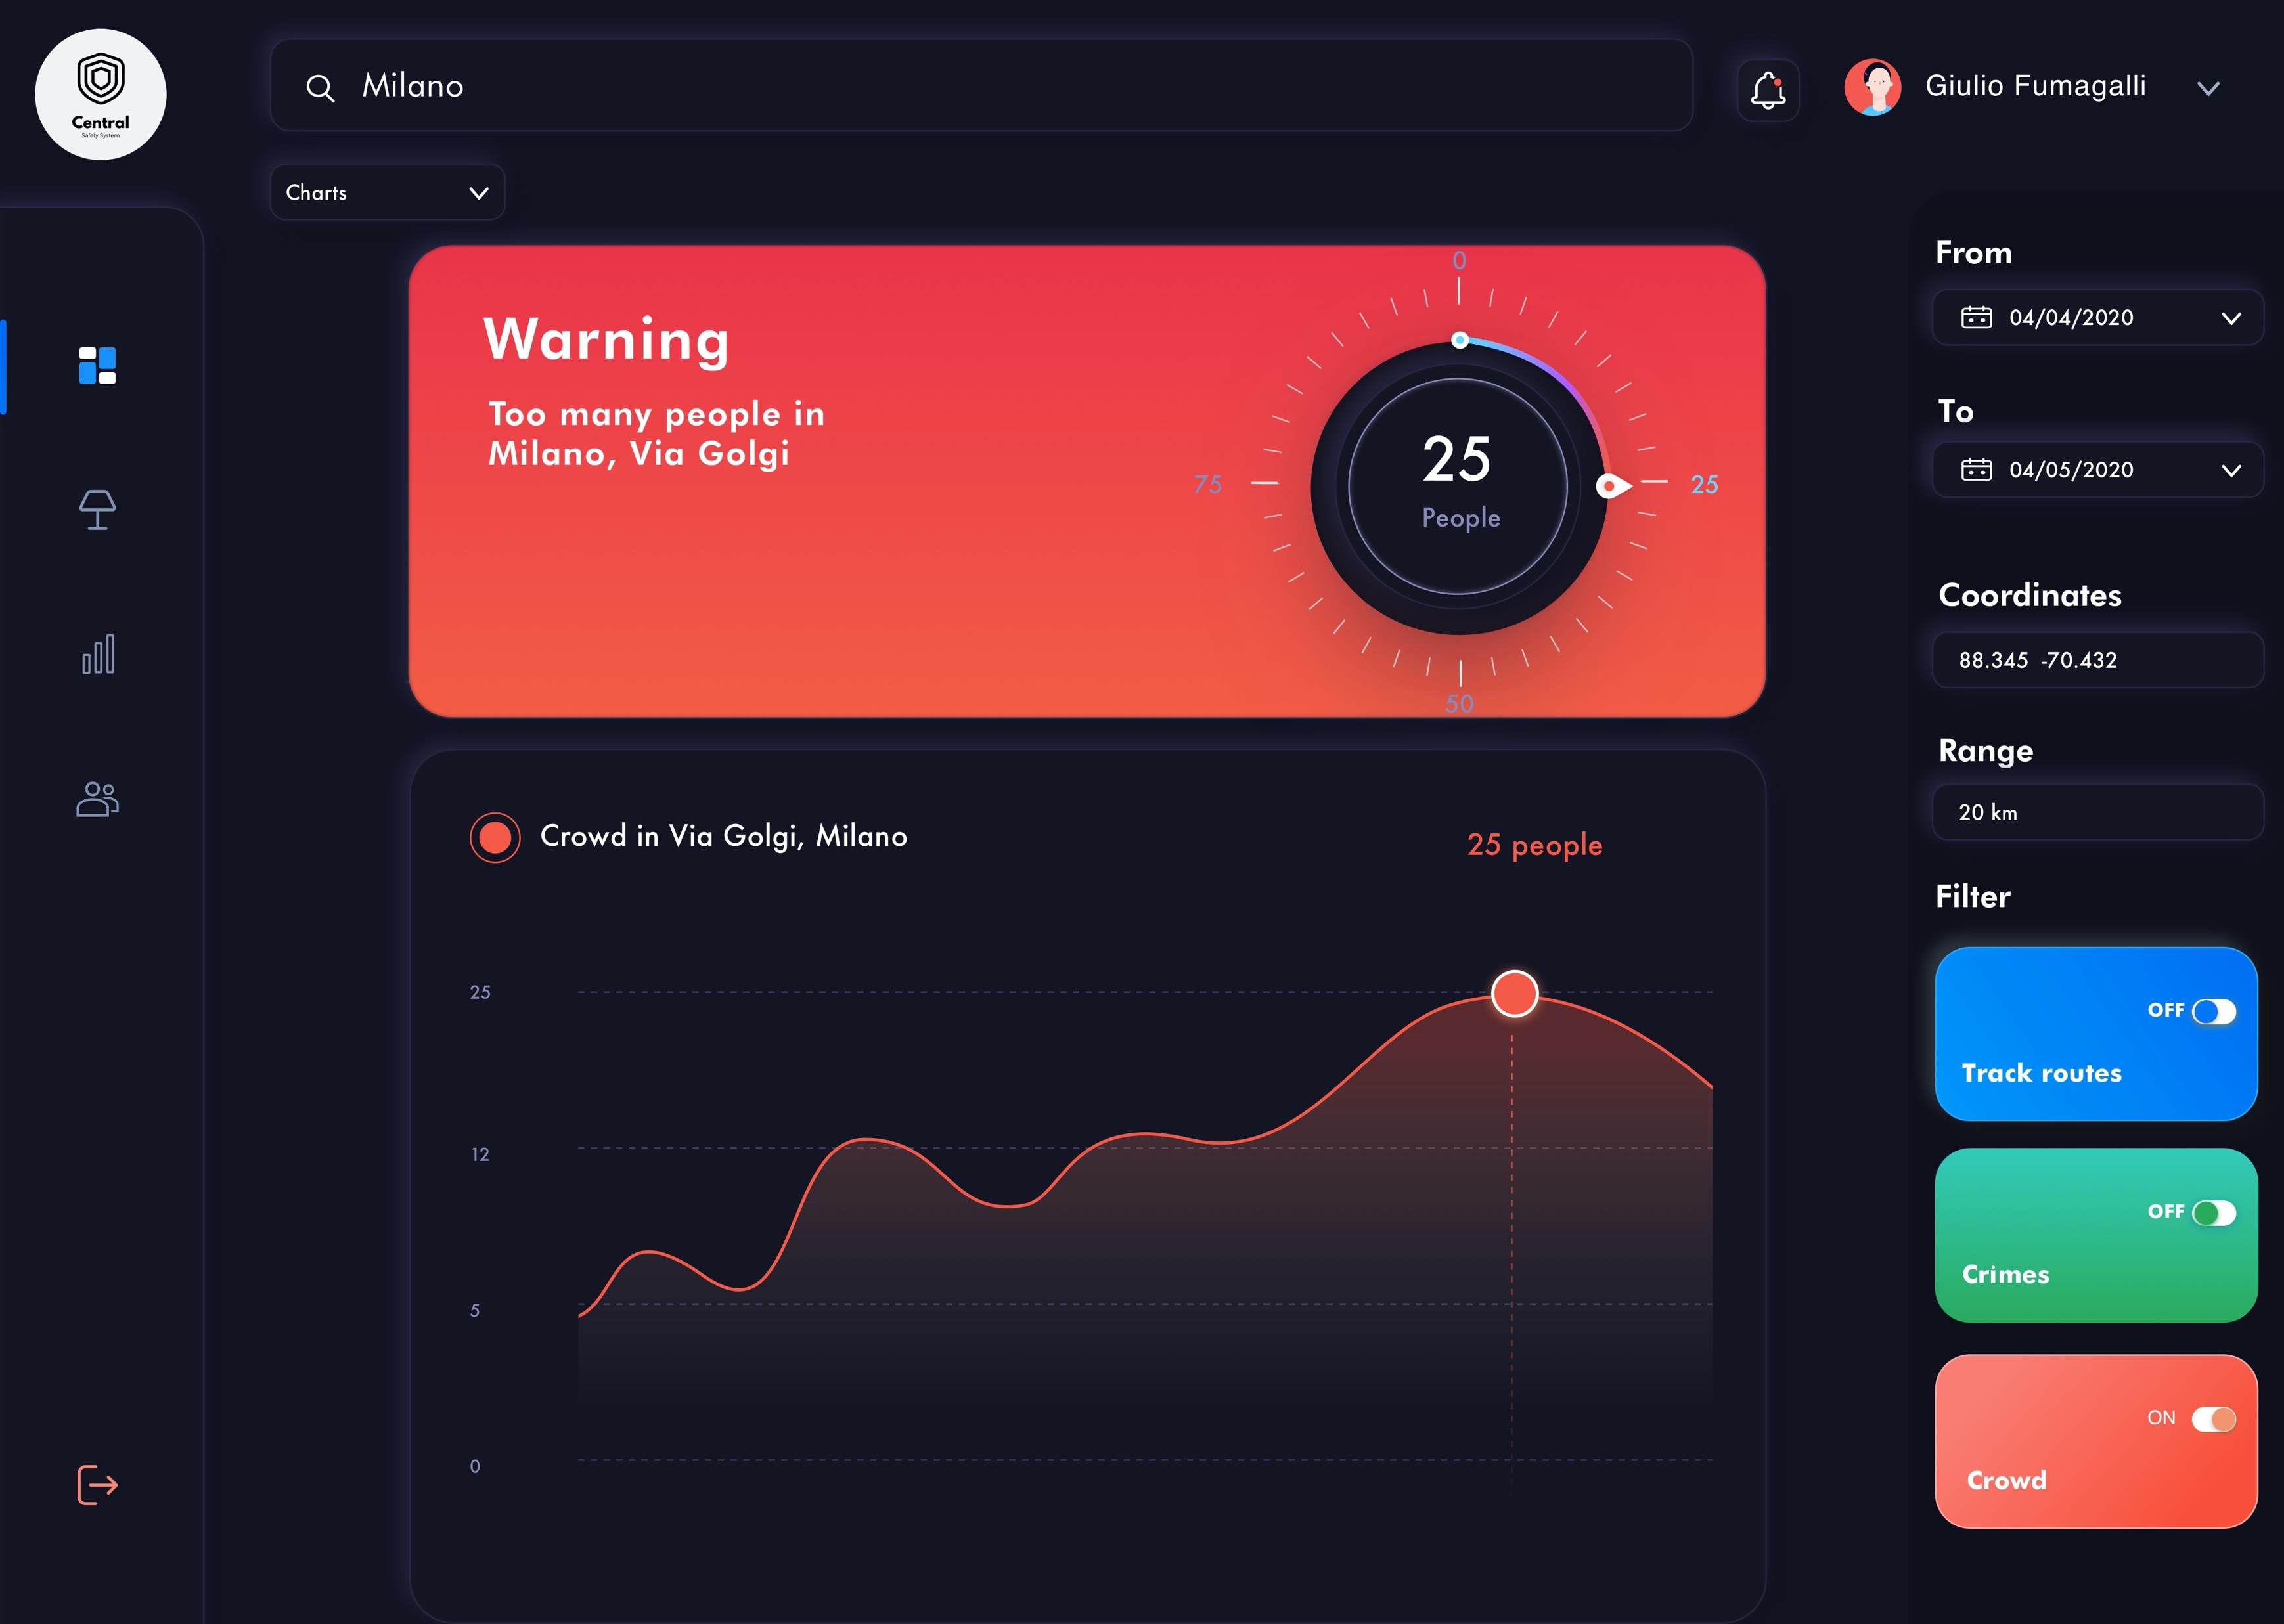
\includegraphics[scale = 0.6]{assets/mockups/mock_dash.png}\\
        \caption[]{Dashboard Page}\label{fig:figure3}
    \end{figure}

\end{document}